\section{The Kokkos Programming Model}\label{chap:kokkosPM}

The Kokkos programming model specifies a language, programming paradigm and an API. The API exposes the machine representation to the developer and defines a set of pattens and types that capture intents and properties of execution. This completes the semantic capture, discussed in Chapter~\ref{chap:background}, We detail all three components as follows.

Kokkos defines a pure interface for C++ and uses C++ as a programming language. This has multiple reasons. It is our experience that application developers of scientific and high-performance computing applications in the high-performance computing community and in industry in general express the demand for C++ and a generic parallel programming model to support their codes. Further, following their estimates, porting efforts towards adapting to vendors, programming models, APIs and software releases represents a burden worth addressing. Lastly, the possibility to maintain pure C++ codes is appealing from the code development and debugging perspective. 

From the programming model perspective, C++ offers template metaprogramming which is well suited to implement generic APIs and libraries. In this case, class specialization and templating allow for compile-type generated types and optimizations for a given hardware architecture. 

Using the programming language, a parallel programming paradigm can be applied to simplify the process of thought. Kokkos supports parallel patterns and tasking. Parallel patterns covers \emph{for}, \emph{scan} and \emph{reduction}. This allows the expression of concurrency over iterative, for-loop computable algorithms. To cover the class of while-loop computable algorithms (irregular algorithms), Kokkos implements the tasking paradigm. Tasks encapsulate work into units that may be executed in parallel to other tasks or sections of the program. Equipped with a language and set of paradigms, a particular set of abstractions can be defined to expose the abstract machine model and capture the intent of the programmer.

To capture semantic information, that is the~\emph{what}, the~\emph{where} and the~\emph{how}, Kokkos introduces six abstractions:~\emph{execution spaces},~\emph{execution patterns},~\emph{execution policies},~\emph{memory spaces},~\emph{memory layout} and~\emph{memory traits}. These abstractions specify semantic information that enable to capture the programmer's intent and allow the runtime to efficiently map the program to any underlying hardware architecture. We list them as follows:
\begin{itemize}
	\item  An execution space is a place where code can be executed. On current hardware architectures this correspond to accelerators and CPUs and can include any compute device in the future. This abstraction supports remote compute devices in distributed memory scenarios as remote execution spaces.
	\item Execution patterns expose the parallel programming paradigm. Supported patterns are \emph{parallel\_for} loop that executes the loop body in any order a specified amount of times, the \emph{parallel\_reduce} which combines a parallel\_for with a reduction operation, \emph{parallel\_scan} which combines a parallel\_for operation with a prefix or postfix scan, and \emph{task} which executes a single function potentially in parallel in respect to other tasks or code sections. 
	\item Execution policy shape the iteration space of a loop pattern. A simple execution policy is a range policy. It specifies that the loop body is executed once for each element in a range.
	\item Memory spaces are the places where data resides. They specify physical locations of data as well as access characteristics. Different physical locations correspond to different device types such as high bandwidth memories, on-die scratch memories or non-volatile bulk storage. Different logical memory spaces allow for concepts such as memory in the CUDA programming model, which is accessible from the host and the CUDA accelerator. Memory spaces, similarly to execution spaces, conceptually support remote memory locations in distributed-memory scenarios. Furthermore, they encapsulate functionality such as consistency control and persistence scopes.
	\item Layouts express the mapping from array indices to address offsets. By adopting appropriate layouts for memory structures, an application can optimize data access patterns in a given algorithm. If an implementation provides polymorphic layouts (i.e. a data structure can be instantiated at compile or runtime with different layouts), architecture-dependent optimizations can be performed.
	\item Memory traits specify how a data structure is accessed. Traits express usage scenarios such as atomic access, random access and streaming loads or stores. This allows the programming model to  optimize load and store operations.
\end{itemize}

\begin{figure}[h]
\begin{Verbatim}[frame=leftline]
Constrained Semantics: Patterns (intent), Spaces, 
Layouts, Policies and Traits
Parallel Paradigms: Parallel patterns and tasking
Expression: Embedded, C++
Control Paradigm: descriptive
\end{Verbatim}
\caption{Semantic capture defined by the Kokkos programming model.}
\label{fig:SemCaptureKokkos}
\end{figure}

\begin{figure}
\begin{Verbatim}[frame=leftline]
template <class ExecPolicy, class FunctorType>
Kokkos::parallel_for(const std::string& name, 
 const ExecPolicy& policy, 
 const FunctorType& functor);
\end{Verbatim}
\caption{The Kokkos~\emph{parallel\_for} class shows how template metaprogramming allows to specialize types. Its descriptive semantic offers the freedom to optimize execution on modern architectures with multiple degrees of concurrency where an execution policy (\emph{ExecPolicy}) shapes the iteration space accordingly.}
\label{fig:parallelFor}
\end{figure}

Figure~\ref{fig:parallelFor} shows one definition of the Kokkos~\emph{parallel\_for} interface. This interface accepts two template parameters and three function arguments. \emph{ExecPolicy} shapes the iteration space for a particular execution space. Examples of execution policies are the~\emph{RangePolicy}, ~\emph{MDRangePolicy} and the~\emph{TeamPolicy}. As the name suggests, these policies express iteration spaces. For example, a range policy defines a one dimensional iteration range. The MDRangePolicy represents a multi-dimensional iteration space and is used to express tightly nested loop patterns. A team policy defines a 1D iteration range, each of which is assigned to a team of threads. This policy allows the expression of hierarchical parallelism. The second template parameter,~\emph{FuntorType}, represent a functor that implements the~\emph{()-operator} with a matching signature for the given execution policy. The functor can be defined using a C++ class, struct or lambda expression. We would like to highlight that the return semantic of the parallel\_for is defined as \emph{potentially asynchronous}. To guarantee a kernel has finished, a developer should call the fence of the execution space on which the kernel is being executed. Otherwise it depends on the execution space where the loop executes and weather this execution space implements a barrier. 

The semantic of the parallel\_for class in Kokkos demonstrates the descriptive nature of the programming model. Programming with patterns and abstractions allows the compiler to generate optimized transformations. 
Generally parallel patterns in Kokkos do not guarantee iteration ordering nor degree of concurrency during their execution. This gives the freedom to the underlying abstraction layers to implement different mapping patterns on different hardware such as assignment of iterations to threads or vector lanes. We believe that these abstraction and their descriptive semantic represent key programming primitives and the way forward for generic support for parallel programming. In conclusion, Figure~\ref{fig:SemCaptureKokkos} shows the semantic capture defined by the Kokkos programming model. Figure~\ref{fig:abstractions} summarizes patterns and abstractions and structures them by information type in the semantic capture.

To the interested reader, the complete programming model description can be accessed on-line\cite{KOKKOS_WIKI}.
The next section shows an example of the Kokkos parallel\_for and explains how it is mapped to the the underlying back-end programming model.

\begin{figure}
\centerline{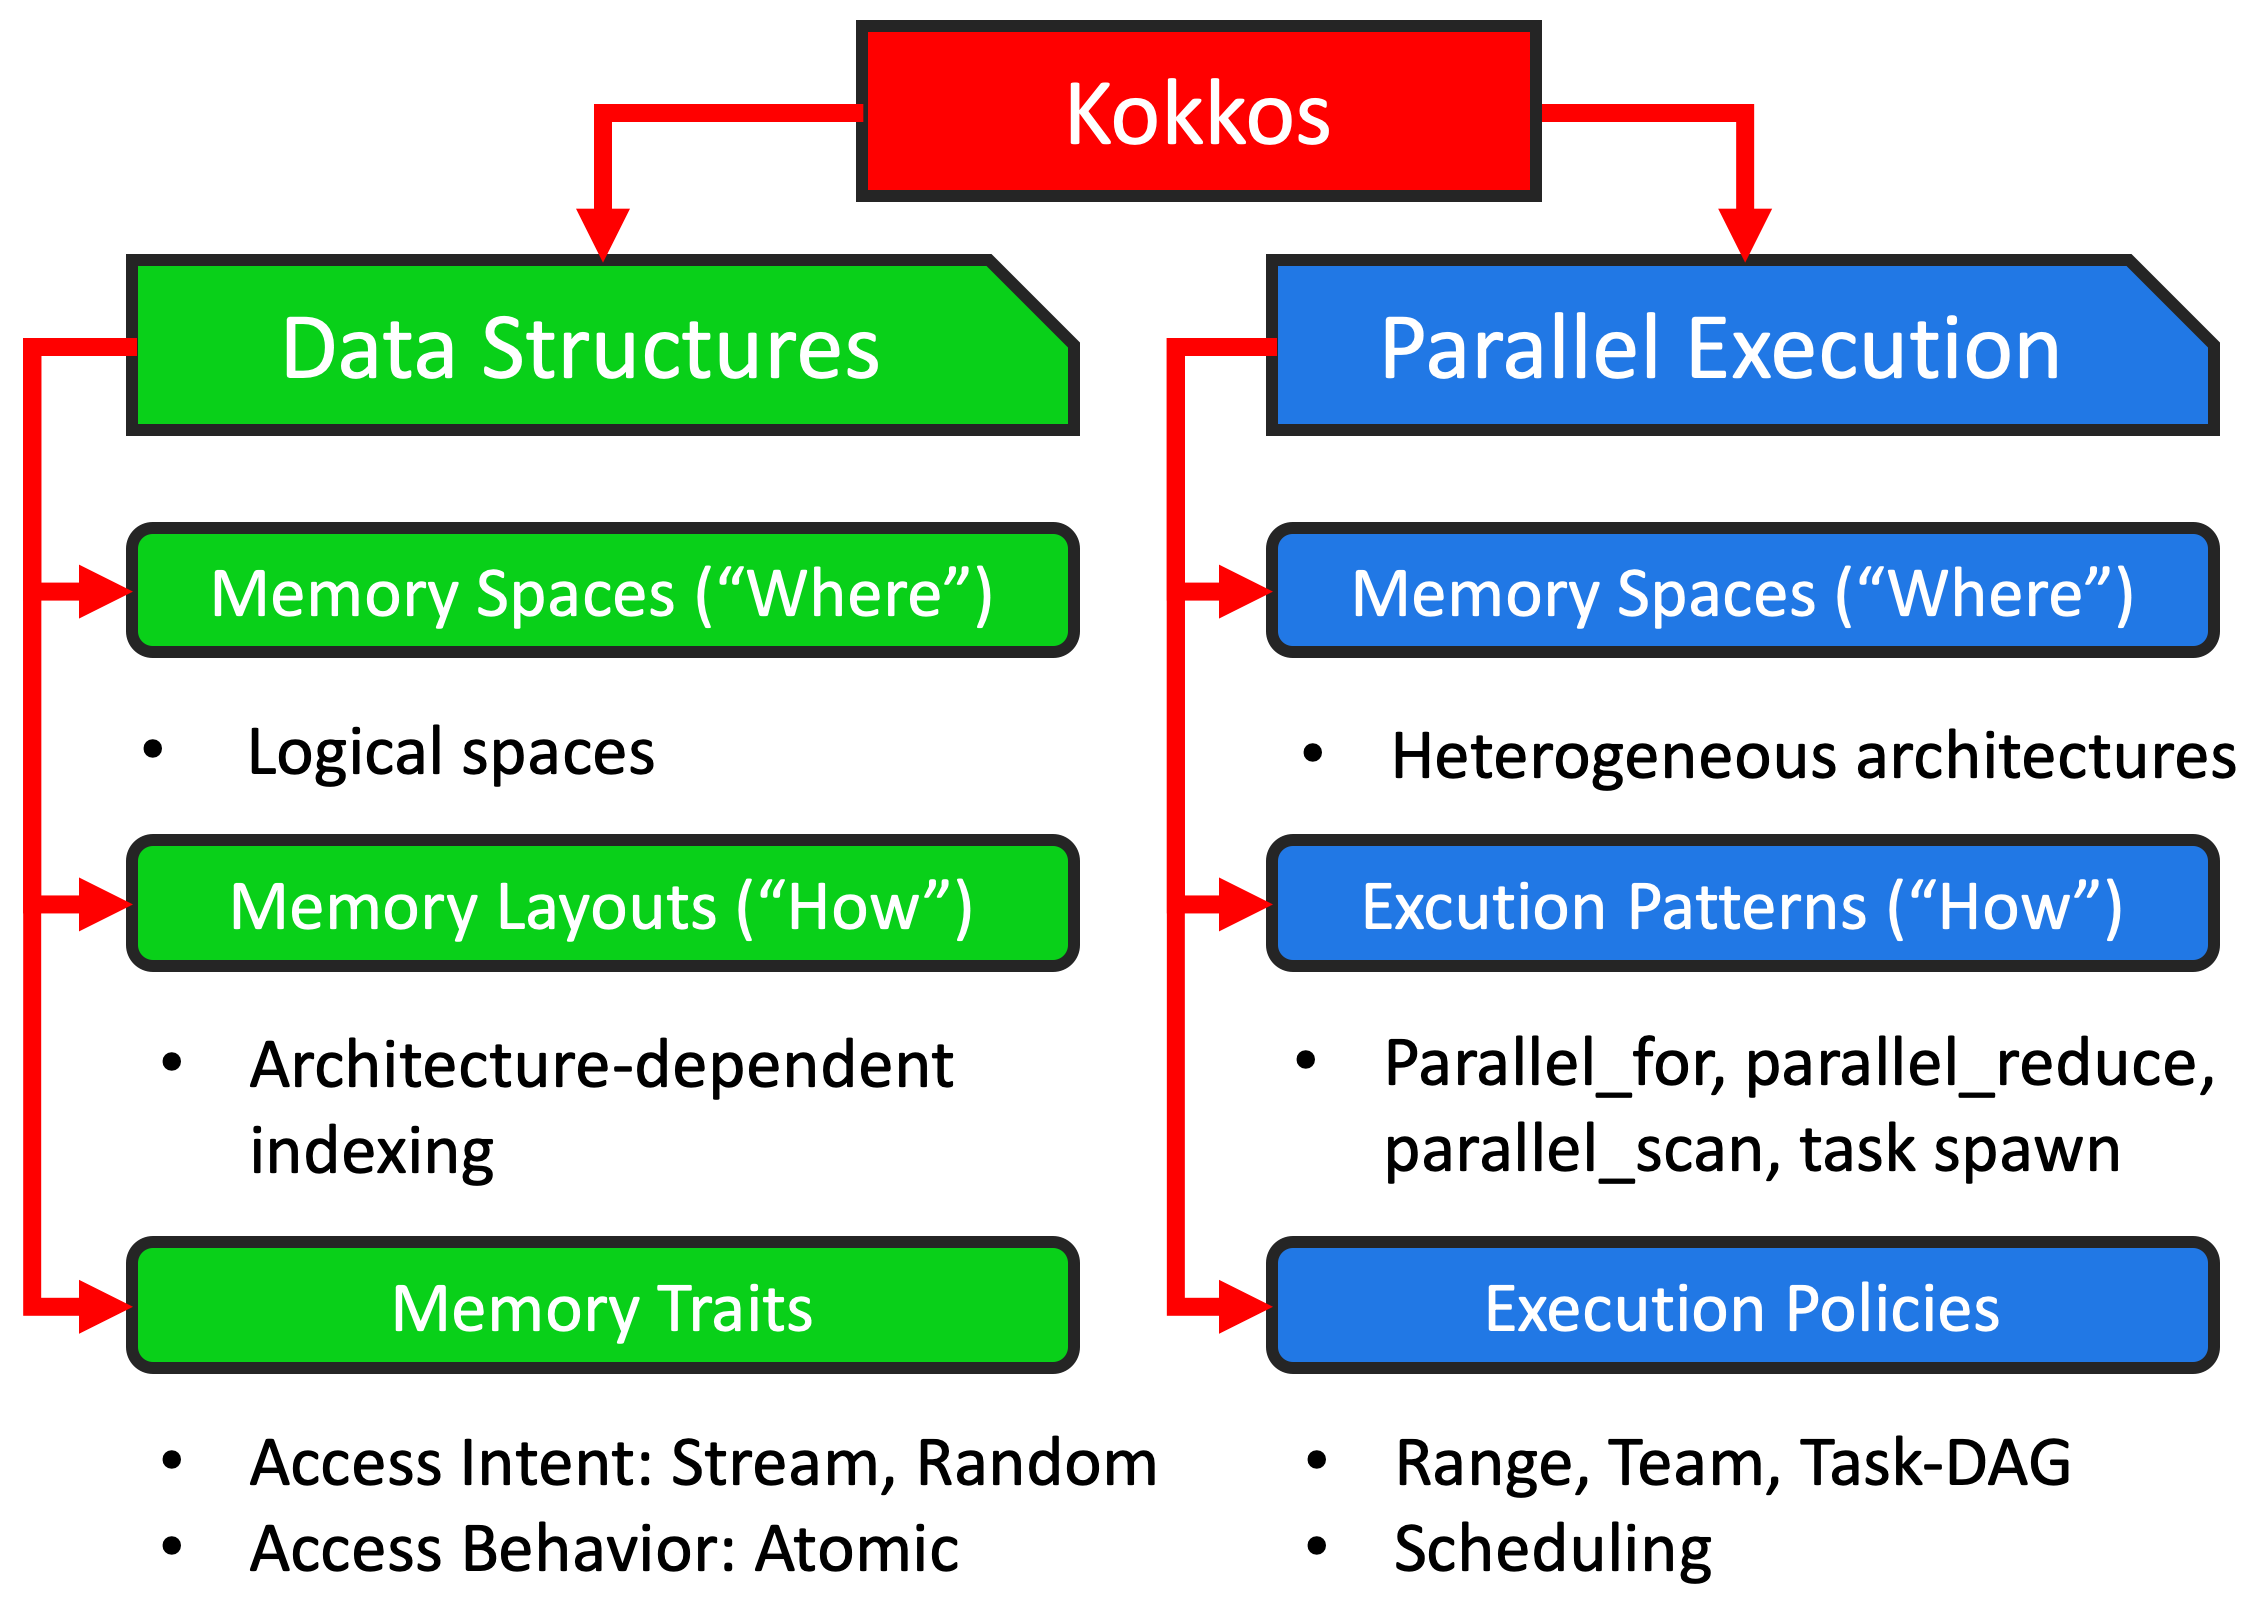
\includegraphics[width=0.45\textwidth]{img/Abstractions.png}}
\caption{Overview of abstractions that define the constrained semantic of the Kokkos parallel programming model.}
\label{fig:abstractions}
\end{figure}
